\chapter{Introducción a los modelos básicos de epidemiología}

\section{Tipos de modelos}

Los modelos discretos (por ejemplo SI, SIR y SIS) usan los estados Susceptible, Infectado y Recuperado. Los nombres suelen hacer referencia al flujo que se sigue para pasar entre los estados. Así, por ejemplo un modelo SI pasa de susceptible a infectado, uno SIR de susceptible a infectado y recuperado y SIS alterna entre susceptible e infectado.

En estos modelos se hacen dos suposiciones:
\begin{enumerate}
\item La población se mezcla de manera homogénea, es decir, todos los individuos tienen la misma probabilidad de contraer la enfermedad.
\item El total de la población es constante.
\end{enumerate}

\subsection{Modelo SI}
Es el modelo más simple de todos, los individuos nacen siendo susceptibles a una enfermedad, una vez infectados no hay tratamiento y permanecen infectados el resto de su vida.
Un ejemplo de una enfermedad que pueda modelarse usando SI es el herpes.

Las siguientes ecuaciones describen el modelo SI:

\begin{equation}
\label{eqn: SI}
\begin{aligned}
S_{n+1}=S_n\left( 1-\frac{\alpha\Delta t}{N}I_n\right) \\
I_{n+1}=I_n\left( 1+\frac{\alpha\Delta t}{N}S_n\right)
\end{aligned}
\end{equation}

donde $S_n$ indica el número de individuos susceptibles en el instante $t_n$, así como $I_n$ hace referencia al número de individuos infectados en ese instante. $\Delta t$ es el tiempo transcurrido entre dos instantes $t_{n+1}-t_n$ y N es el tamaño total de la población, con condiciones iniciales $S_0>0$, $I_0>0$ y $S_0+I_0=N$.

En estas ecuaciones $\alpha$ es la tasa de contacto, esto es, el número medio de individuos con los que un infectado tiene suficiente contacto para contagiarlo en un intervalo de tiempo. Por tanto, $S_n$ representa el número de individuos susceptibles en el tiempo $n\Delta t$.

Ahora, imponemos las suposiciones descritas anteriormente para estos modelos. En primer lugar, suponemos que la población se mezcla de manera homogénea de ahora en adelante, y para la segunda: La población total se mantiene constante, que es trivial que se cumpla siempre, ya que sumando el sistema de ecuaciones el resultado es $N$ y asumimos que las soluciones son siempre positivas pues las soluciones negativas no tienen sentido.
Además, no tiene sentido hablar de un número negativo de individuos, ya sean infectados, recuperados o susceptibles de contraer la enfermedad, luego para imponer que las ecuaciones tengan soluciones positivas una condición necesaria y suficiente para $S_n$ es que $\alpha\Delta t \leq 1$.

\begin{proof}
Supongamos que $I_n, S_n > 0$. Por la segunda ecuación del modelo (\ref{eqn: SI}) es claro que $I_{n+1}>0$, pues $S_n>0$ y $1+\frac{\alpha\Delta t}{N}>0$.

Para la primera ecuación tenemos que 
$$S_{n+1}>0 \Leftrightarrow 1-\frac{\alpha\Delta t}{N}I_n >0$$

ya que $I_n$ es positivo por hipótesis. Esto equivale a:
$$N>\alpha\Delta t(N-I_n) \Leftrightarrow \alpha\Delta t I_n > (\alpha\Delta t -1) N$$

Como $\alpha\Delta t I_n > 0$, tenemos entonces que la desigualdad se da si y solo si:
$$\alpha\Delta t -1 <0 \Leftrightarrow \alpha\Delta t \leq 1$$
\end{proof}


Buscamos ahora ver cuál es el comportamiento del sistema, calculando los puntos de equilibrio, para lo que resolvemos:

$$
\begin{cases}
S^*=S^*\left( 1-\frac{\alpha\Delta t}{N}I^*\right) \\
I^*=I^*\left( 1+\frac{\alpha\Delta t}{N}S^*\right) \\
S^*+I^*=N
\end{cases}
$$

Los únicos puntos de equilibrio posibles son: $S^*=0, I^*=N$ y $S^*=N, I^*=0$, y como sabemos que tenemos condiciones iniciales positivas y es claro que $S_n$ es monótonamente decreciente e $I_n$ es monótonamente creciente, ya que $S_{n+1}$ es $S_n$ multiplicado por un valor menor que $1$, mientras que $I_{n+1}$ corresponde a $I_n$ multiplicado por un valor mayor que $1$, así $S_{n+1}<S_n$ y $I_{n+1}>I_n$ para cualquier $n\in\mathbb{N}$, entonces debe converger a $S^*=0, I^*=N$, pues son sucesiones monótonas acotadas.

Expresando $\alpha$ como una tasa podemos obtener las ecuaciones diferenciales análogas de la siguiente manera:

$$\frac{S_{n+1} - S_n}{\Delta t} \approx S'(t),$$

luego su análoga continua es:

\begin{equation}
\begin{aligned}
S'(t) = -\frac{\alpha}{N}SI \\
I'(t) = \frac{\alpha}{N}SI
\end{aligned}
\end{equation}

con condiciones iniciales $S(0)+I(0)=N$.

De manera análoga al caso discreto, es decir, suponiendo las funciones constantes y resolviendo el sistema de ecuaciones, podemos comprobar que este sistema converge a $S^*=0, I^*=N$ y, por tanto, tiene el mismo comportamiento que el caso discreto.

\textcolor{red}{RESOLVER, VIENE EN EL ARTICULO}
Sustituyendo en el modelo $S=N-I$ obtenemos la ecuación diferencial logística

$$I'(t) = \frac{\alpha}{N}(N-I).$$

Esta ecuación diferencial se puede resolver por separación de variables como sigue:

\textcolor{red}{He hecho las cuentas y no me sale la misma solución que en el pdf del artículo, no sé si me he equivocado, aunque el límite sí coincide}

\begin{equation}
\begin{aligned}
I'(t)=\frac{\alpha}{N}(N-I(t)) & \Leftrightarrow \int \frac{dI}{N-I} = \int dt \frac{\alpha}{N} \\
& \Leftrightarrow -\log(N-I) = \frac{\alpha}{N}t+c \\
& \Leftrightarrow  \frac{1}{N-x} = e^{\frac{\alpha}{N}t+c} \\
& \Leftrightarrow  I(t) = N-\frac{1}{e^{\frac{\alpha}{N}t+c}}
\end{aligned}
\end{equation}

Ahora usando el valor inicial $I(0)$ tenemos:

\begin{equation}
\begin{aligned}
I(0) = N-\frac{1}{e^c} & \Leftrightarrow e^c = \frac{1}{N-I(0)} \\
& \Leftrightarrow c=\log(\frac{1}{N-I(0)}
\end {aligned}
\end{equation}

luego la solución general es:

$$I(t) = N-\frac{N-I(0)}{e^{\frac{\alpha}{N}t}}$$


\begin{figure}
\begin{center}
\caption{Gráfica del modelo SI, en una población total de $100$ individuos, con valores iniciales $S_0=99, I_0 = 1, \alpha = 0.1, T_0 = 0, T = 100$.}
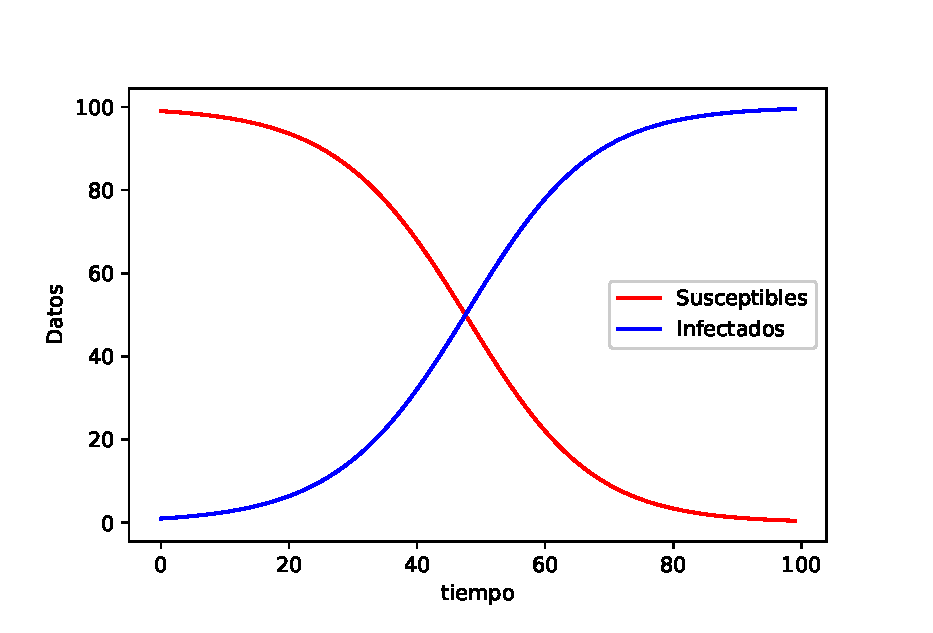
\includegraphics[scale=1]{graficaSI}
\end{center}
\end{figure}

\subsection{Modelo SIR}
Comienza como el SI, pero tras infectarse los individuos pasan a un estado Recuperado, en el cual no pueden infectarse ni infectar a otros.
Por ejemplo, la varicela. 

El modelo es el siguiente:

\begin{equation}
\label{eqn: SIR_modelo}
\begin{aligned}
S_{n+1} = & S_n \left(1-\frac{\alpha\Delta t}{N} I_n \right) \\
I_{n+1} = & I_n \left( 1-\gamma \Delta t + \frac{\alpha\Delta t}{N} S_n \right) \\
R_{n+1} = & R_n + \gamma \Delta t I_n
\end{aligned}
\end{equation}

con condiciones iniciales $S_0>0$, $I_0>0$, $R_0\geq 0$, satisfaciendo $S_0+I_0+R_0=N$.

En estas ecuaciones, de nuevo tenemos que $\alpha$ es la tasa de contacto, esto es, el número medio de individuos con los que un infectado tiene suficiente contacto para contagiarlo en un intervalo de tiempo y $\gamma$ es la probabilidad de que un infectado pase a recuperado/retirado/aislado/fallecido en un intervalo de tiempo, con $\alpha >0$ y $\gamma >0$.

Se supone que la población permanece constante, $S_n+I_n+R_n=N$.

Además, tenemos que las soluciones a este sistema discreto son positivas para cualquier valor de las condiciones iniciales si, y solo si:

$$\max{\big\{\gamma\Delta t, \alpha\Delta t\big\} } \leq 1$$

\textcolor{red}{Aqui falta la demostracion de esto}

o equivalentemente:

$$\min{\bigg\{ \frac{1}{\gamma}, \frac{1}{\alpha} \bigg\} } \geq \Delta t$$

Por tanto, el intervalo de tiempo debe ser menor que el tiempo medio requerido para un contacto exitoso y menor que el período medio infeccioso.
% Con contacto exitoso asumo que se refiere al tiempo necesario para infectar a un individuo. Sí es esto confirmado por la profe

El comportamiento global del sistema es fácil de ver. Definimos como $\mathcal{R}=S_0 \alpha/(N\gamma )$ la tasa reproductiva. El valor de $\mathcal{R}$ determina el comportamiento global del modelo. \textcolor{red}{(a esto después lo llamo tasa de transmisión media en el artículo \cite{demongeotSIEpidemicModel})}. 

Notemos que $S_n$ es estrictamente decreciente y $R_n$ es estrictamente creciente. Estudiémoslas:

Sea $S_\infty=\lim_{n\rightarrow\infty} S_n\geq 0$, cuyo límite existe pues es una sucesión estrictamente decreciente y acotada inferiormente por $0$, que depende de las condiciones iniciales. Si $S_0\leq \frac{\gamma N}{\alpha}$, o, equivalentemente, $\mathcal{R}\leq 1$ entonces $I_1\leq I_0$ y, como $S_n$ es estrictamente decreciente, tenemos que $I_{n+1}\leq I_n$, es decir, no hay epidemia. En otro caso, tenemos $S_0> \frac{\gamma N}{\alpha}$, entonces $I_1>I_0$. Debe ocurrir que $S_\infty <\frac{N\gamma}{\alpha}$, pues si no fuera así, tendríamos que $I_n$ crece hacia un equilibrio, $I_\infty$, lo que implica que $R_n$ se aproxima a infinito cuando $n\rightarrow\infty$, lo cual no es posible. Así, el número de infectados finalmente comienza a decrecer y se aproxima a $0$. Además, sabemos por el Lema 1 de \cite{allenDiscretetimeSISIR1994} que $S_\infty>0$.

El modelo continuo se comporta de la misma forma que el modelo discreto, este sería:

\begin{equation}
\label{eqn: modelo_SIR_continuo}
\begin{cases}
S'(t) = -\dfrac{\alpha}{N}SI \\
I'(t) = I\left(d\frac{\alpha}{N}S-\gamma \right) \\
R'(t) = R+\gamma I
\end{cases}
\end{equation}

donde $S(0)+I(0)+R(0)=N$. La tasa reproductiva en este caso es $\mathcal{R}=S(0)\alpha /(N\gamma )$, y si $\mathcal{R}\leq 1$  no hay epidemia, pero en cambio, si es mayor, hay epidemia.

\begin{figure}
\begin{center}
\caption{Gráfica del modelo SIR, en una población total de $100$ individuos, con valores iniciales $S_0=99, I_0 = 1, R_0 = 0, \alpha = 0.1, \gamma = 0.01 T_0 = 0, T = 300$.}
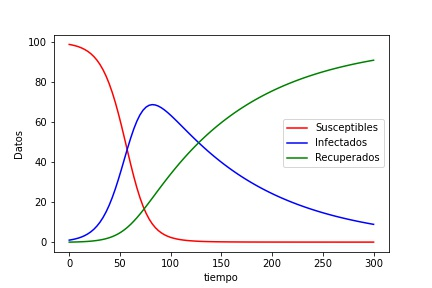
\includegraphics[scale=1]{graficaSIR}
\end{center}
\end{figure}


\subsection{Modelo SIS}
Es similar al SI, pero tras infectarse los individuos vuelven a ser susceptibles.
Por ejemplo, los resfriados pueden modelarse usando SIS.

El modelo es una perturbación del modelo SI visto antes, es el siguiente:

\begin{equation}
\label{eqn: modelo_SIS}
\begin{aligned}
S_{n+1} = S_n \left(1-\frac{\alpha\Delta t}{N} I_n \right) + \gamma \Delta t I_n \\
I_{n+1} = I_n \left( 1-\gamma \Delta t + \frac{\alpha\Delta t}{N} S_n \right)
\end{aligned}
\end{equation}

con condiciones iniciales positivas $S_0>0$, $I_0>0$ cumpliendo $S_0+I_0=N$. Por lo tanto, el tamaño de la población es constante.

En estas ecuaciones, $\alpha$ de nuevo representa la tasa de contacto, esto es, el número medio de individuos con los que un infectado tiene suficiente contacto para contagiarlo en un intervalo de tiempo y $\gamma$ es la probabilidad de que un infectado pase a recuperado/retirado/aislado/fallecido en un intervalo de tiempo, donde se cumple $\alpha >0$ y $\gamma >0$.

Además las soluciones siempre son positivas si, y solo si:

$$\gamma \Delta t \leq 1 $$ y $$\alpha\Delta t< \left( 1+\sqrt{\gamma \Delta t} \right)^2$$

Esto se puede consultar en el Lema 2 del Apéndice de \cite{allenDiscretetimeSISIR1994}.

\textcolor{red}{No he comprobado las cuentas de esas condiciones}

La tasa reproductiva de este modelo se define como $\mathcal{R}=\alpha /\gamma$ \textcolor{red}{No entiendo como saca esa tasa reproductiva, he repetido las cuentas y las de antes estaban mal. Si no es por definición como dijimos el otro día no se dónde sale}

Si $\mathcal{R}\leq 1$ entonces se tiene que $I_{n+1} < I_n$, ya que $0<S_n<N$ y las soluciones son positivas. En este caso es fácil ver que el límite, al ser una sucesión monótona decreciente y acotada inferiormente, es $(S^*,I^*)=(N,0)$. Supongamos que $S^*<N$, entonces existen $n_1, \epsilon$ tales que para todo $n \geq n_1$:
$$S_n<S^*+\epsilon < N$$
y usando las ecuaciones (\ref{eqn: modelo_SIS})
$$I_{n+1} \leq I_n \left( 1-\gamma \Delta t + \frac{\alpha\Delta t}{N} S_n \right) = \rho I_n$$

Como $\rho < 1$ tenemos que $I^*=0$, lo que contradice que $S^*<N$.

Si $\mathcal{R}>1$ realizando la sustitución $S_n=N-I_n$ y el cambio

$$x_n=\frac{\alpha \Delta t I_n}{N(1+\alpha \Delta t - \gamma \Delta t)}$$

tenemos:

\begin{equation}
\begin{aligned}
x_n=\frac{\alpha \Delta t I_n}{N(1+\alpha \Delta t - \gamma \Delta t)} \Leftrightarrow \\
\alpha\Delta t I_n = x_nN(1+\alpha\Delta t-\gamma\Delta t) \Leftrightarrow \\
I_n = \frac{x_nN(1+\alpha\Delta t - \gamma\Delta t}{\alpha\Delta t}
\end{aligned}
\end{equation}

entonces sustituyendo:

\begin{equation}
\begin{aligned}
\frac{x_{n+1}N(1-\alpha\Delta t-\gamma\Delta t)}{\alpha \Delta t} = \frac{x_nN(1+\alpha\Delta t-\gamma \Delta t)}{\alpha\Delta t}\left( 1-\gamma\Delta t+\frac{\alpha\Delta t}{N}\left(N-\frac{x_nN(1+\alpha\Delta t-\gamma\Delta t)}{\alpha\Delta t}\right) \right)
\end{aligned}
\end{equation}

Despejando de esta expresión:

\begin{equation}
\begin{aligned}
x_{n+1} & = x_n\left( 1-\gamma\Delta t+\frac{\alpha\Delta t}{N}N-\frac{\alpha\Delta t}{N}\frac{x_nN(1+\alpha\Delta t -\gamma \Delta t)}{\alpha\Delta t} \right) \\
& = x_n(1-\gamma\Delta t + \alpha\Delta t -x_n(1+\alpha\Delta t -\gamma\Delta t)) \\
& = x_n((1-\gamma\Delta t+\alpha\Delta t)(1-x_n))
\end{aligned}
\end{equation}

luego obtenemos la ecuación logística

$$x_{n+1} = (1+\alpha \Delta t - \gamma \Delta t)x_n(1-x_n)$$

Entonces la restricción necesaria para garantizar soluciones positivas no es suficiente para asegurar la convergencia, en este caso a dicha restricción hay que añadir la condición $\alpha \Delta t \leq 2+\gamma \Delta t$ \textcolor{red}{Esta condición supongo que viene de alguna condición conocida de la ecuación logística que no recuerdo, ups. A partir de aquí me pierdo un poco, está en el último párrafo de la página 10 del artículo de Allen}


 







\section{Cosas del articulo de rsos que no sé que nombre ponerles}

\subsection{Introducción}

Estimar la tasa de transmisión media es uno de los aspectos más cruciales en epidemiología. Esta tasa condiciona la fase de la epidemia e incluso si va a extinguirse. Es combinación de tres factores:

\begin{enumerate}
\item Coeficiente de virulencia: Relacionado con el agente infeccioso.
\item Coeficiente de susceptibilidad: Relacionado con el anfitrión.
\item Número de contactos por unidad de tiempo entre individuos.
\end{enumerate}

Los dos primeros factores se tienen en cuenta a la vez en la probabilidad de transmisión.

Todos los factores pueden cambiar con el tiempo, el primero debido a mutaciones del virus y los dos últimos por medidas de contención. Por tanto, observar el decrecimiento de la transmisión media en una enfermedad es una buena forma de comprobar la efectividad de las medidas de contención.

Consideramos un modelo SI modificado con el objetivo de compararlo con los datos obtenidos en la pandemia de la COVID-19 hasta el momento y así tratar de predecir su comportamiento en el futuro.

El modelo SI continuo es el siguiente:

\begin{equation}
\label{eqn: SI_cont}
\begin{aligned}
S'(t) = -\tau (t)S(t)I(t) \\
I'(t) = \tau (t)S(t)I(t) -vI(t)
\end{aligned}
\end{equation}

donde $S(t)$ es el número de individuos susceptibles , $I(t)$ el número de individuos infectados en el tiempo $t$ y $\tau (t)$ la tasa de transmisión, que combina el número de contactos por unidad de tiempo y la probabilidad de transmisión. Además, notemos que $v$ es constante, donde $1/v$ es la duración media del período de infección, y $vI(t)$ el flujo de individuos recuperados o fallecidos. %vI(t) es el flujo de recuperados o muertos porque ha mezclado el modelo SI y SIR; vI(t) serian los recuperados, pero se ahorra la ecuacion de la R

$$S(t_0)=S_0>0, \: I(t_0)=I_0>0$$

Ahora, consideramos que al final del período infeccioso nos han informado de una fracción del total de casos, en este caso $f\in (0,1]$. Sea $C_R(t)$ el número total (acumulado) de casos reportados. Entonces:

\begin{equation}
\label{eqn: acumulada}
C_R(t) = {C_R}_0 + vfC_I(t) \; \forall t \geq t_0
\end{equation}

\textcolor{red}{¿Por qué $vfC_I(t)$ va multiplicado por $v$?}

donde

$$C_I(t) = \int_{t_0}^t I(w) dw $$

Asumimos conocidos $S_0 > 0$, $1/v>0$, $f\in (0,1]$. Por tanto, queremos averiguar $I_0$, $\tau (t)$.

\subsection{Aproximando $I_0$ y $\tau (t_0)$}
Ahora, procedemos a intentar aproximar $I_0$ y $\tau (t_0)$:

Al comienzo de la pandemia podemos asumir que $S(t)$ y $\tau (t)$ son constantes e iguales a $S_0$ y $\tau_0 = \tau (t_0)$ respectivamente. Así, sustituyendo estos valores en la ecuación (\ref{eqn: SI_cont}) obtenemos:

$$I'(t) = (\tau_0 S_0 -v) I(t)$$.

Resolviendo la ecuación diferencial llegamos a:

$$I(t) = I_0\exp{((\tau_0 S_0-v)(t-t_0))}$$.

Sustituyendo en (\ref{eqn: acumulada}):

$$C_R(t) = {C_R}_0 + vfI_0\frac{\mathrm{e}^{(\tau_0 S_0 -v)(t-t_0)} -1}{\tau_0 S_0-v}$$

Así, hemos obtenido un primer modelo para los casos acumulados al principio de la pandemia.

Reescribimos la ecuación como:

\begin{equation}
\label{eqn: acumulada_modelo}
C_R(t) = \chi_1 \mathrm{e}^{\chi_2 t} -\chi_3
\end{equation}

Estimamos $\chi_3$ usando los datos de la epidemia obtenidos, y el mejor ajuste para los datos es $\chi_3=0$.

Ahora, usando (\ref{eqn: acumulada}) y (\ref{eqn: acumulada_modelo}) tenemos:

\begin{equation}
I_0=\frac{\chi_1\chi_2\mathrm{e}^{\chi_2 t_0}}{vf}
\end{equation}

Y, como de reescribir sabemos que $\chi_2 = \tau_0 S_0-v$, entonces

\begin{equation}
\tau_0 = \frac{\chi_2+v}{S_0}
\end{equation}

Si suponemos que $\tau (t) = \tau_0$ constante, tenemos que el modelo queda:

\begin{equation}
\begin{aligned}
S'(t) = -\tau_0S(t)I(t) \\
I'(t) = \tau_0S(t)I(t) -vI(t)
\end{aligned}
\end{equation}

Usando la ecuación de $S(t)$ y resolviéndola obtenemos:

$$S(t) = S_0\exp{\left( -\tau_0 \int_{t_0}^t I(w) dw \right)} = S_0\exp{(-\tau_0 C_I(t))}$$

Ahora, sustituyendo esta expresión en la ecuación de $I(t)$ del modelo y usando $C_I'(t)=I(t)$:

$$I'(t) = S_0\exp{\left( -\tau_0 C_I(t)\right) }\tau_0 C_I'(t)-vI(t)$$

Finalmente, integrando entre $t_0$ y $t$ tenemos que:

$$I(t)=C_I'(t)=I_0+S_0(1-\exp{(-\tau_0 C_I(t)}))-vC_I(t)$$
 
Observamos entonces que el número total de infectados es monótono creciente, ya que $I(t)>0$ siempre por positividad de las soluciones y $C_I'(t)=I(t)>0$. Cabe destacar que esto no implica que el número de infectados sea monótono creciente.

\begin{theorem}
Sea $t>t_0$ fijo. El número de infectados acumulados es estrictamente creciente respecto a las siguiente cantidades:
\begin{itemize}
\item $I_0>0$ Número inicial de infectados
\item $S_0>0$ Número inicial de individuos susceptibles.
\item $\tau>0$ Tasa de transmisión
\item $1/v$ Tiempo medio de la infección.
\end{itemize}
\end{theorem}

\subsection{Fórmula teórica para $\tau (t)$}

Usando la ecuación del modelo inicial (\ref{eqn: SI_cont}) obtenemos:
% La ecuacion de la S$

$$S(t) = S_0 \exp{\left( - \int_{t_0}^t \tau(w) I(w) dw \right) } $$ 

Ahora, sustituyendo en la ecuación (\ref{eqn: SI_cont}):
% La ecuacion de la I

$$I'(t) = S_0 \exp{\left( - \int_{t_0}^t \tau(w) I(w) dw \right) } \tau (t) I(t) -vI(t) $$

Integramos en ambos lados entre $t_0$ y $t$, luego:

$$ C_I'(t) = I_0 + S_0 \left( 1-\exp{\left(- \int_{t_0}^t \tau (w) I(w)dw \right)}\right) -vC_I(t)$$

Equivalentemente, por (\ref{eqn: acumulada}):

$$C_R'(t) = vf\left( I_0 + S_0 \left( 1-\exp{\left(- \frac{1}{vf}\int_{t_0}^t \tau (w ) I(w)dw \right)}\right)\right) +v{C_R}_0 -vC_R(t)$$

\textcolor{red}{Esta cuenta no termina de salirme, pero tiene más o menos sentido}

Así, obtenemos el Teorema 3.1 de \cite{demongeotSIEpidemicModel}, que nos da la relación directa buscada.

\textcolor{blue}{He estado leyendo el resto del artículo, en el que habla de obtener una expresión explícita de $\tau (t)$ e $I_0$, pero para eso usan datos de China en específico y ajustes por ordenador, así que no tengo muy claro si merece la pena incluir esa parte ya que no tenemos los datos y por tanto sería fiarse un poco de lo que han hecho ellos}







